\documentclass[17pt]{beamer} %Makes presentation
%\documentclass[handout]{beamer} %Makes Handouts
\usetheme{Singapore} %Gray with fade at top
\useoutertheme[subsection=false]{miniframes} %Supppress subsection in header
\useinnertheme{rectangles} %Itemize/Enumerate boxes
\usecolortheme{seagull} %Color theme
\usecolortheme{rose} %Inner color theme

\definecolor{light-gray}{gray}{0.75}
\definecolor{dark-gray}{gray}{0.55}
\setbeamercolor{item}{fg=light-gray}
\setbeamercolor{enumerate item}{fg=dark-gray}

\setbeamertemplate{navigation symbols}{}
%\setbeamertemplate{mini frames}[default]
%\setbeamercovered{dynamics}
\setbeamerfont*{title}{size=\Large,series=\bfseries}
\setbeamerfont{footnote}{size=\tiny}

%\setbeameroption{notes on second screen} %Dual-Screen Notes
%\setbeameroption{show only notes} %Notes Output

\setbeamertemplate{frametitle}{\vspace{.5em}\bfseries\insertframetitle}
\newcommand{\heading}[1]{\noindent \textbf{#1}\\ \vspace{1em}}

\usepackage{bbding,color,multirow,times,ccaption,tabularx,graphicx,verbatim,booktabs}
\usepackage{colortbl} %Table overlays
\usepackage[english]{babel}
%\usepackage[latin1]{inputenc}
%\usepackage[T1]{fontenc}
\usepackage{lmodern}

%\author[]{Thomas J. Leeper}
\institute[]{
  \inst{}%
  Department of Government\\London School of Economics and Political Science
}

\usepackage{tikz}
\usetikzlibrary{shapes,arrows}

\title{Causal Mechanisms and Process Tracing}

% Aside from knowing that one thing (X) caused another thing (Y), we often want to know how that causal process worked. This is the study of ``causal mechanisms''. How do we study causal mechanisms to gain a deeper understanding of causal relationships in politics? How do we study the process by which a causal effect plays out?


\date[]{}

\begin{document}

\frame{\titlepage}

\frame{\tableofcontents}



\section{Review}
\frame{\tableofcontents[currentsection]}

\frame{
	\frametitle{Review Case Studies}
	\begin{itemize}\itemsep0.5em
	\item Many uses of case studies
	\item In case comparisons (last week), we focused on scoring cases on variables to test theories \textit{between cases}
	\end{itemize}
}

\frame{

Theory testing involves:

\begin{itemize}
\item Between-case comparisons, or 
\item \textbf<2>{Across-time comparisons}, or 
\item Between-case \& across-time comparisons
\item Within-case comparisons at a lower level of analysis
\end{itemize}

}



\frame{}

\section{Mechanisms}
\frame{\tableofcontents[currentsection]}


\frame<1>[label=causality]{
\frametitle{{\normalsize Four (or five) principles of causality\footnote{From Kellstedt and Whitten}}}
\begin{enumerate}\itemsep0.5em
\item Correlation
\item Nonconfounding
\item Direction (``temporal precedence'')
\item \textbf<2->{Mechanism}
\item (Appropriate level of analysis)
\end{enumerate}
}


\frame<1-6>[label=causalgraph]{
	\begin{center}
	\tikzstyle{dot} = [minimum size=1pt]
	\tikzstyle{arrow} = [->, very thick]
	\begin{tikzpicture}
        \node<1->[dot, label={[label distance=0.05cm]270:D}] at (0,0) (D) {};
        \fill<1-> (D) circle [radius=3pt];
        \node<1->[dot, label={[label distance=0.05cm]270:Y}] at (5,0) (Y) {};
        \fill<1-> (Y) circle [radius=3pt];
        \draw<1-6>[arrow] (D) -- (Y);
        
        \node<2->[dot, label={[label distance=0.05cm]90:A}] at (4,3) (A) {};
        \fill<2-> (A) circle [radius=3pt];
        \draw<2->[arrow] (A) -- (Y);
        \node<3->[dot, label={[label distance=0.05cm]270:B}] at (-2,-1) (B) {};
        \fill<3-> (B) circle [radius=3pt];
		\draw<3->[arrow] (B) -- (D);
        
        \node<4->[dot, label={[label distance=0.05cm]90:Z}] at (-3,4) (Z) {};
        \fill<4-> (Z) circle [radius=3pt];
		\draw<4->[arrow] (Z) -- (D);
        \draw<4->[arrow] (Z) -- (Y);
        % confounding
        \node<5>[dot, label={[label distance=0.05cm]90:Z}] at (-3,4) (Z) {};
        \fill<5> (Z) circle [radius=3pt, fill=blue];
        \draw<5>[arrow, color=red] (Z) -- (D);
        \draw<5>[arrow, color=red] (Z) -- (Y);
        \node<5> at (1,4) (conf) {{\color{red} Confounding}};
        
        \node<7->[dot, label={[label distance=0.05cm]270:M}] at (2.5,0) (M) {};
        \fill<7-> (M) circle [radius=3pt];
        \draw<7->[arrow] (D) -- (M);
        \draw<7->[arrow] (M) -- (Y);
        
        \node<8-9>[dot, label={[label distance=0.05cm]270:M}] at (2.5,0) (M) {};
        \fill<8-9> (M) circle [radius=3pt, fill=blue];
        \draw<9>[arrow, color=red] (D) -- (M);
        \draw<9>[arrow, color=red] (M) -- (Y);
    \end{tikzpicture}
    \end{center}
}

% causality is complicated; graphs allow us to represet theories visually
% it helps us to identify factors that may be causally relevant



\againframe{causality}

\frame{
\frametitle{Mediators/Mechanisms}

\small

\begin{itemize}
\item Definition: ``the generative mechanism through which the focal independent variable is able to influence the dependent variable of interest'' \footnote{p. 1173 from Baron, R.M., and Kenny, D.A. 1986. ``The Moderator-Mediator Variable Distinction in Social Psychological Research: Conceptual, Strategic, and Statistical Considerations.'' \textit{Journal of Personality and Social Psychology} 51(6): 1173--1182.}
\item Dropping the tautology, ``the pathway(s) or process(es) by which an effect is produced''
\item Allows us to distinguish:
	\begin{itemize}
	\item \textit{Direct} effects
	\item \textit{Indirect} effects
	\end{itemize}
\end{itemize}
}
% define mechanism
% synonyms: mediator, causal pathway, ``how'' of a causal effect
% thinking about mechanisms allow us to talk about direct and ``mediated'' effects
% that is to say: how are cause and outcome linked causally?

\againframe<6-10>{causalgraph}


\frame{
\frametitle{Two Uses of Studying Mechanisms}
\begin{enumerate}\itemsep1em
\item Determine \textit{how} a causal effect comes about
\item Establish seemingly disconnected cause and outcome through a chain of smaller causal effects
\end{enumerate}
}

\frame{

\frametitle{1. The \textit{how} of the \textit{why}}

\begin{itemize}
\item A causal effect is an explanation of \textit{why} something occurs
\item Mechanisms explain \textit{how} that effect occurs
\end{itemize}

}

% a mechanism may not be obvious
% there may also be multiple mechanisms

\frame{

\frametitle{Example: Smoking}

\begin{columns}
  \begin{column}{0.4\textwidth}
    We know that smoking kills.\\
    
    \vspace{1em}
    
    \textit{How} does this effect occur?
    
  \end{column}
  \begin{column}{0.4\textwidth}
    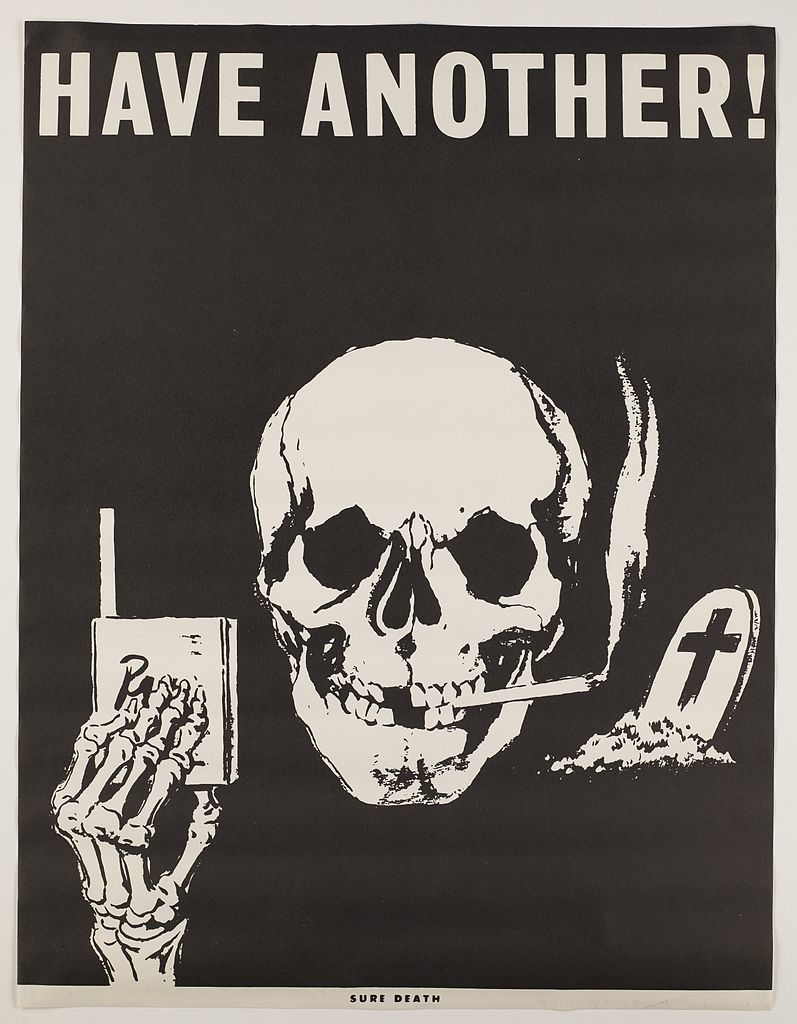
\includegraphics[width=1.2\columnwidth]{images/smoking}\\    
    {\tiny Source: \copyright{} \href{http://wellcomeimages.org/indexplus/image/L0074423.html}{Wellcome Trust}}
  \end{column}
\end{columns}


}

% draw a causal graph on the board

% smoking -- ? -- death
% smoking -- lung cancer -- death
% smoking -- intake of toxins -- lung cacer -- death
% smoking -- intake of toxins -- dna mutation -- lung cancer -- death

% smoking -- heart disease -- death
% smoking -- oxidants -- inflammation -- reduced blood flow -- heart disease -- heart attack -- death
% smoking -- nicotine uptake -- increase heart rate -- oxygen demand
% smoking -- nicotine update -- hypertension -- heart attack -- death

\frame{

\frametitle{2. Sum of small effects}

\begin{itemize}\itemsep0.5em
\item We may be able to establish a number of small linkages
\item The product (multiplication) of these effects is the \textit{total effect}
\item<2-> Two ways to conceptualize this:
	\begin{itemize}
	\item Deterministic causality
	\item Probabilistic causality
	\end{itemize}
\end{itemize}

}

% link back to cancer example
% Morgan and winship are especially interested in situations where we don't know if X causes Y (e.g., smoking and cancer)
% but where we can observe pieces of that causal chain that might allow us to add up to a link between smoking and cancer


% talk about deterministic causality: each step being necessary for the next step to be possible
% versus probabilistic causality (or deterministic but heterogeneous causal effects): each step increases the value of the next step




\frame<1-5>{

\frametitle{{\large Pearl's Front Door Criterion}}

% Pearl's ``front door criterion'' we can learn how X affects Y if we have an exhaustive and isolated set of mechanisms

% add a graph


\begin{columns}
  \begin{column}{0.55\textwidth}
    
    \small
    
    \begin{itemize}
    \item Same rules for understanding mechanisms as causes generally
    \item Mechanisms must be:
	    \begin{itemize}
	    \item \textbf<3>{exhaustive}
	    \item \textbf<4>{isolated}
	    \end{itemize}
    \end{itemize}
    
  \end{column}
  \begin{column}{0.4\textwidth}
  
  	\tikzstyle{arrow} = [->, very thick]
  	\begin{tikzpicture}
        \node<1->[label={[label distance=0.05cm]270:{\footnotesize D}}] at (0,0) (D) {};
        \fill<1-> (D) circle [radius=2pt];
        \node<1->[label={[label distance=0.05cm]0:{\footnotesize Y}}] at (3,0) (Y) {};
        \fill<1-> (Y) circle [radius=2pt];
          
        \node<1>[label={[label distance=0.05cm]270:{\footnotesize M}}] at (1.5,0) (M) {};
        \fill<1> (M) circle [radius=2pt];
        \draw<1>[arrow] (D) -- (M);
        \draw<1>[arrow] (M) -- (Y);

		% two mechanisms
		\node<2,4>[label={[label distance=0.05cm]270:{\footnotesize M1}}] at (1.5,-0.5) (M1) {};
		\node<3>[label={[label distance=0.01cm]90:{\footnotesize M1}}] at (1.5,-0.5) (M1) {};
		\fill<2-> (M1) circle [radius=2pt];
        \node<2->[label={[label distance=0.05cm]90:{\footnotesize M2}}] at (1.5,0.5) (M2) {};
        \fill<2-> (M2) circle [radius=2pt];
        \draw<2->[arrow] (D) -- (M1);
        \draw<2->[arrow] (M1) -- (Y);
        \draw<2->[arrow] (D) -- (M2);
        \draw<2->[arrow] (M2) -- (Y);	
          
        % non-exhaustive
        \node<3>[draw, circle, inner sep=0pt, minimum size=6pt, label={[label distance=0.05cm]270:{\footnotesize M3}}] at (1.5,-2) (M3) {};
        %\fill<3> (M3) circle [radius=3pt];
        \draw<3>[arrow] (D) -- (M3);
        \draw<3>[arrow] (M3) -- (Y);
        \draw<3>[arrow] (M3) -- (M1);
          
        % mechanism confound
        \node<4>[draw, circle, inner sep=0pt, minimum size=6pt, label={[label distance=0.05cm]180:{\footnotesize Z}}] at (0,2) (Z) {};
        %\fill<4> (Z) circle [fill=white, radius=2pt];
        \draw<4>[arrow] (Z) -- (D);
        \draw<4>[arrow] (Z) -- (M2);

      \end{tikzpicture}
    
  \end{column}
\end{columns}
}

\frame{}


\frame{
\frametitle{Do We Care About Mechanisms?}

Write for two minutes

\begin{itemize}\itemsep0.5em
\item Is understanding a mechanism necessary for causal inference?
\item When should we be satisfied that we have ``bottomed out'' a causal process?
\end{itemize}
}

% do we care about mechanisms? how deep do we want to go into a mechanism?
% when are we satisfied that we have ``bottomed out'' a mechanism?

% if concepts have many parts and we theorize that it is one part of that concept that transmits a causal effect, should we ever study causality at the level of concepts or should we only study causality at the level of the constitutive attribute that is thought to be causally relevant?



\section{Process Tracing}
\frame{\tableofcontents[currentsection]}

\frame{

\frametitle{Process Tracing}

\begin{itemize}\itemsep0.5em
\item Definition: ``analysis of processes of change that seeks to uncover causal mechanisms and causal sequences''\footnote{p.300 from Brady, H.E., and Collier, D. 2004. \textit{Rethinking Social Inquiry}. Rowman \& Littlefield.}
\item Single-case method
\item Focused on gathering CPOs
\item Sequence of counterfactuals
\end{itemize}

}


% at its most basic level, it answers ``what happened?'' (i.e., it is descriptive history)
% the difference, however, is that it is about causal inference, which is implicitly about within-case counterfactuals
% generally, these are treated with a deterministic perspective on causality (if this hadn't happened, what would have happened instead?)

% application of logic and ``counterfactual'' method
% update beliefs about counterfactuals in sequence

% inductive versus deductive approach
% process tracing as a standalone method versus as a supplement to other methods
	% for example, often use very aggregated data to establish a relationship and process tracing to document how it comes about

\frame{
\frametitle{{\large Causal Process Observations}}

\normalsize

\begin{itemize}\itemsep0.5em
\item Definition: ``An insight or piece of data that provides information about the context, process, or mechanism, and that contributes distinctive leverage in causal inference''\footnote{Brady and Collier 2004, p.277}
\item Might be used to:
	\begin{itemize}
	\item Inductively generate hypotheses
	\item Deductively test a chain of causal relationships
	\end{itemize}
\end{itemize}
}



\frame{
\frametitle{Inductive Process Tracing}

\begin{columns}
  \begin{column}{0.55\textwidth}

	\begin{itemize}\itemsep0.5em
	\item Broad search for sequential steps necessary for an event to occur
	\item No \textit{a priori} expectations to test
	\item Analogous to detective work
	\end{itemize}
	
    
  \end{column}
  \begin{column}{0.4\textwidth}
    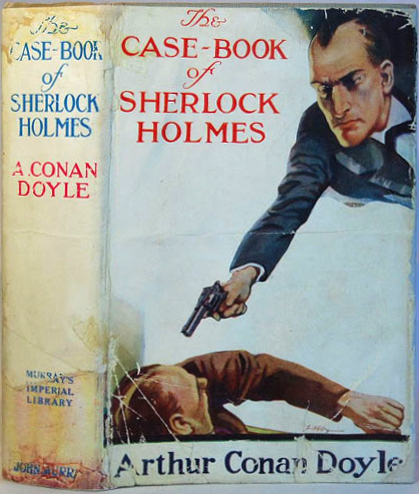
\includegraphics[width=\columnwidth]{images/sherlockholmes}
    
    {\tiny Source: Public Domain}
  \end{column}
\end{columns}


}

% class examples: Sherlock Holmes stories are process-tracing tests of how murders (or other crimes) that link a potential cause (a murderer) to an outcome (a death) via a series of causal steps that leave behind pieces of evidence



\frame{
\frametitle{Deductive Process Tracing}

\begin{itemize}\itemsep1em
\item Sequence of within-case hypothesis tests
\item Theory or extant evidence guide chosen comparisons
	\begin{itemize}
	\item May iterate if there is no or very weak evidence for one's hypothesis(es)
	\end{itemize}
\end{itemize}
}

% Example: smoking and cancer


\frame{
\frametitle{{\large Four Process Tracing Tests\footnote{Note: I am not a fan of this typology.}}}

Broadly consistent with Neyman-Pearson hypothesis testing.

\begin{enumerate}
\item Straw-in-the-wind test
\item Hoop test
\item Smoking gun test
\item Doubly decisive test
\end{enumerate}

}
% reason I do not like it is that it is difficult to specify a priori whether something is one of these types of tests
% part of process-tracing is not knowing what you're looking for, let alone whethere that evidence will or will not be consistent with expectations




\frame{
\frametitle{Major Caveat: Uncertainty}

\begin{itemize}\itemsep0.5em
\item Our uncertainty is a function of $n$
\item<2-> Process-tracing is a single-case design
	\begin{itemize}
	\item Reduce uncertainty by finding within-case variation
	\item Accept only high certainty about specific case % but high uncertainty about the general class of cases of which this case is a member
	\end{itemize}
\item<3-> Can we gather within-case DSOs at a lower level of analysis to better understand causality?
	\begin{itemize}
	\item<4-> Local-level geographical variation
	\item<4-> Across-time variation
	\end{itemize}
\end{itemize}

}


\appendix
\frame{}

\end{document}
